\input{../macros.tex}
\renewcommand{\note}[1]{}
\renewcommand{\answerbox}[1]{}
\begin{document}
\homework{\textbf{Week 5 Worksheet \color{blue} Solutions}}{Designing Information Systems and Devices I}{\textbf{Spring 2020}}{}{}
\problem{1: Introduction to Circuit Components}
\\
\note{
Introduction to basic circuit components.
Mentors: do a mini lecture on what is charge, what is voltage, and what is current. See lecture notes for definitions. 
}

In this problem, we will introduce the fundamental circuit components. 

\begin{enumerate}

\item{
What is a voltage source?
}

\sol{
Firstly, a voltage source is represented in this manner: 
\begin{center}
    \begin{circuitikz}
        \draw(0,0)
	    to[V=$V$] ++(1,0);
    \end{circuitikz}
\end{center}

A voltage source \textbf{guarantees} that the potential at its positive end will be $V$ more than the potential at its negative end, no matter what. 
}

\item{
 What is a current source?  
}

\sol{
A current source is represented in this manner: 
\begin{center}
    \begin{circuitikz}
        \draw(0,0)
	     to[I, l=$I$] ++(1,0);
    \end{circuitikz}
\end{center}
A current source \textbf{guarantees} that the current passing through the unit in the direction of the arrow will be its designated value. 
}

\item{What is voltage? What is a voltage drop?}

\sol{
For our discussion, it suffices to think of voltage as a kind of driver for current. Current is the movement of charges. A voltage difference forces current to move from the point (node) that has higher voltage, to the point that has lower voltage. 

Voltage drop is the voltage lost (decline of nodal voltage) across a circuit component. 
}

\item{Consider the figure below. If $V_1 \neq V_2$, what will happen to the circuit?

\begin{center}
    \begin{circuitikz}
    \draw(0,4)
	%to[short] ++(0,-1)
	to[V_=$V_1$] ++(0,-4)
	to[short] node[ground] {} ++(0,-1);
	
	\draw(0,4)
	to[short] ++(2,0)
	to[V_=$V_2$] ++(0,-4)
	to[short] ++(-2,0);
    \end{circuitikz}
\end{center}

}

\sol{
Let us designate the potential at the positive end of $V_1$ to be $V^+_1$, the potential at the negative end of $V_1$ to be $V^-_1$, the potential at the positive end of $V_2$ to be $V^+_2$, and the potential at the negative end of $V_2$ to be $V^-_2$. $V^-_1$ and $V^-_2$ are equal to 0 because of the ground. Then, the potential across $V_1$ is $V^+_1$, and the potential across $V_2$ is $V^+_2$. Since $V^+_1$ and $V^+_2$ are connected by a wire, they must be the same voltage; we know that a wire does not affect a circuit's behavior, so the voltage must stay constant across it. 
This means that $V^+_1 = V^+_2$. However, we know that the voltage potential $V^+_1 - V^-_1$ is not equal to $V^+_2 - V^-_1$ as given in the question. Hence, we see that we cannot have two voltage sources connected in this configuration.
}

\item {What happens in this case if $I_1 \neq I_2$?
\begin{center}
    \begin{circuitikz}
    \draw(0,0) 
    to[I=$I_1$] ++(0,2)
    to[I=$I_2$] ++(0,2);
    \end{circuitikz}
\end{center}
}

\sol{
The current source at the bottom guarantees that through that wire there will be $I_1$ current going through, and the current source at the top guaranteed that $I_2$ current goes through that wire. This is a contradiction, and is not theoretically possible in a circuit. 

Also, look at the point in between the two current sources. $I_1$ enters on one end, and $I_2$ leaves on the other end. This is impossible.
}

\item{
What is a resistor? 
}

\sol{
A resistor is represented in this manner: 
\begin{center}
	\begin{circuitikz}

	\draw(0,0)
	to[R, v=$ $, i=$ $] ++(3,0);
	\end{circuitikz}
	\end{center}
A resistor is a circuit unit designed to `resist' the flow of current. Following convention, there is a ``voltage drop'' across a resistor from the positive end to the negative end. The voltage drop across a resistor is $V_R = I_R R$, where $V_R$ is the voltage drop, $I_R$ is the current through the resistor and $R$ is the resistance of the resistor. 
}

\item{What is power?}

\sol{
Power is the rate at which work is done, where work is in terms of electrical energy.

For circuits, the power \textit{consumed} or \textit{dissipated} by a device is $P = IV$, where the current and voltage abide by passive sign convention.

\textbf{Common Misconceptions:}
\begin{itemize}
	\item Active components do not necessarily dissipate negative power! Consider the following circuit:
	\begin{center}
		\begin{circuitikz}
			\draw
			(0,0) node[ground] () {}
				to[V=$1\si{\volt}$, invert] ++(0,2)
				to[R=$1\si{\ohm}$] ++(2,0)
			(2,0) node[ground] () {}
				to[V=$2\si{\volt}$, invert] ++(0,2);
		\end{circuitikz}
	\end{center}
	When calculating the power dissipated by the LHS voltage source, we see the current flows counterclockwise about the circuit. With passive sign convention, we calculate the power $P_{V_1} = 1\si{\volt} \times 1\si{\ampere}$, which is positive! The left-side voltage source is dissipating power.
\end{itemize}
}

\end{enumerate}
\newpage
\problem{2: Passive Sign Convention}
\\
% Lydia Lee, Spring 2019
% lydia.lee@berkeley.edu
For the following components, label all the missing $V_\text{element}$, $I_\text{element}$, and +/- signs. \textit{Hint: The value of the voltage and current sources shouldn't affect passive sign convention---remember that voltage and current can be negative!}

\note{For parts (a) and (b), make sure to clarify to your students that the box figure can represent any arbitrary circuit element (a resistor, a voltage source, etc.).}

\begin{enumerate}
\item{
\begin{center}
	\begin{circuitikz}[scale=0.75]
		\ctikzset{resistor = european}
		\draw (0,0) to[R, v=$V_\text{element}$] ++(4,0);
	\end{circuitikz}
\end{center}
}
\sol{
\begin{center}
	\begin{circuitikz}[scale=0.75]
		\ctikzset{resistor = european}
		\draw (0,0) to[R, v=$V_\text{element}$, i=$I_\text{element}$] ++(5,0);
	\end{circuitikz}
\end{center}
}

\item{
\begin{center}
	\begin{circuitikz}[scale=0.75]
		\ctikzset{resistor = european}
		\draw (0,0) to[R, i=$I_\text{element}$] ++(5,0);
	\end{circuitikz}
\end{center}
}
\sol{
\begin{center}
	\begin{circuitikz}[scale=0.75]
		\ctikzset{resistor = european}
		\draw (0,0) to[R, v=$V_\text{element}$, i=$I_\text{element}$] ++(5,0);
	\end{circuitikz}
\end{center}
}

\item{
\begin{center}
	\begin{circuitikz}[scale=0.75]
		\draw 
		(0,0) to[V, v=$V_\text{S}$, invert] ++(0,3)
			to[open] ++(.5,0)
			to[open, v^=$V_\text{element}$] ++(0,-3);
	\end{circuitikz}
\end{center}
}
\sol{
\begin{center}
	\begin{circuitikz}[scale=0.75]
		\draw 
		(0,0) to[V, v=$V_\text{S}$, i=$I_\text{element}$, invert] ++(0,3)
			to[open] ++(.5,0)
			to[open, v^=$V_\text{element}$] ++(0,-3);
	\end{circuitikz}
\end{center}
}

\item{
\begin{center}
	\begin{circuitikz}[scale=0.75]
		\draw 
		(0,0) to[V, v=$1\si{\volt}$, invert] ++(0,3)
		(0,0) to[open] ++(.5,0)
			to[open, v_=$V_\text{element}$] ++(0,3);
	\end{circuitikz}
\end{center}
}

\note{If students are confused by this answer, draw the source on the board, then a box around it. Shade in the box so the voltage source is obscured, and now the problem is identical to having a black box voltage source. This particular style of question has featured on several exams, and it's good to have lots of practice with this when calculating power.
}

\sol{
\begin{center}
	\begin{circuitikz}[scale=0.75]
		\draw 
		(0,0) to[V, v=$1\si{\volt}$, invert] ++(0,3)
		(0,0) to[open] ++(.5,0)
			to[open, v_=$V_\text{element}$] ++(0,3)
		(0,0) to[open, i=$I_\text{element}$, invert] ++(0,3);
	\end{circuitikz}
\end{center}
}

\item{ 
\begin{center}
	\begin{circuitikz}[scale=0.75]
		\draw 
		(0,0) to[V, v=$V_\text{S}$, i=$I_\text{element}$, invert] ++(0,3);
	\end{circuitikz}
\end{center}
}
\sol{
\begin{center}
	\begin{circuitikz}[scale=0.75]
		\draw 
		(0,0) to[V, v=$V_\text{S}$, i=$I_\text{element}$, invert] ++(0,3)
			to[open] ++(.5,0)
			to[open, v^=$V_\text{element}$] ++(0,-3);
	\end{circuitikz}
\end{center}
}

\newpage
\item{
\begin{center}
	\begin{circuitikz}[scale=0.75]
		\draw 
		(0,0) to[V, v=$-1\si{\volt}$, invert] ++(0,3)
		(0,0) to[open, i=$I_\text{element}$, invert] ++(0,3);
	\end{circuitikz}
\end{center}
}
\sol{
\begin{center}
	\begin{circuitikz}[scale=0.75]
		\draw 
		(0,0) to[V, v=$-1\si{\volt}$, invert] ++(0,3)
		(0,0) to[open] ++(.5,0)
			to[open, v_=$V_\text{element}$] ++(0,3)
		(0,0) to[open, i=$I_\text{element}$, invert] ++(0,3);
	\end{circuitikz}
\end{center}
}

\item{\textbf{(PRACTICE)}

\begin{center}
	\begin{circuitikz}[scale=0.75]
		\draw 
		(0,0) to[I, l=$I_\text{S}$, invert] ++(0,3)
			to[open] ++(.5,0)
			to[open, v^=$V_\text{element}$] ++(0,-3);
	\end{circuitikz}
\end{center}
}
\sol{
\begin{center}
	\begin{circuitikz}[scale=0.75]
		\draw 
		(0,0) to[I, l=$I_\text{S}$, invert] ++(0,3)
			to[open] ++(.5,0)
			to[open, v^=$V_\text{element}$] ++(0,-3)
		(0,3) to[open, i^=$I_\text{element}$] ++(0,-3);
	\end{circuitikz}
\end{center}
}

\item{\textbf{(PRACTICE)}

\begin{center}
	\begin{circuitikz}[scale=0.75]
		\draw 
		(0,0) to[I, l=$I_\text{S}$, invert] ++(0,3)
		(0,0) to[open] ++(.5,0)
			to[open, v_=$V_\text{element}$] ++(0,3);
	\end{circuitikz}
\end{center}
}
\sol{
\begin{center}
	\begin{circuitikz}[scale=0.75]
		\draw 
		(0,0) to[I, l=$I_\text{S}$, invert] ++(0,3)			
		(.5,0) to[open, v_=$V_\text{element}$] ++(0,3)
		(0,0) to[open, i^=$I_\text{element}$] ++(0,3);
	\end{circuitikz}
\end{center}
}

\item{\textbf{(PRACTICE)}

\begin{center}
	\begin{circuitikz}[scale=0.75]
		\draw 
		(0,0) to[I, l=$I_\text{S}$, invert] ++(0,3)
			to[open, i=$I_\text{element}$] ++(0,-3);
	\end{circuitikz}
\end{center}
}
\sol{
\begin{center}
	\begin{circuitikz}[scale=0.75]
		\draw 
		(0,0) to[I, l=$I_\text{S}$, invert] ++(0,3)
			to[open, i=$I_\text{element}$] ++(0,-3)
		(.5,3) to[open, v^=$V_\text{element}$] ++(0,-3);
	\end{circuitikz}
\end{center}
}

\item{\textbf{(PRACTICE)}

\begin{center}
	\begin{circuitikz}[scale=0.75]
		\draw 
		(0,0) to[I, l=$I_\text{S}$, invert] ++(0,3)
		(0,0) to[open, i=$I_\text{element}$, invert] ++(0,3);
	\end{circuitikz}
\end{center}
}
\sol{
\begin{center}
	\begin{circuitikz}[scale=0.75]
		\draw 
		(0,0) to[I, l=$I_\text{S}$, invert] ++(0,3)
		(0,0) to[open] ++(.5,0)
			to[open, v_=$V_\text{element}$] ++(0,3)
		(0,0) to[open, i=$I_\text{element}$, invert] ++(0,3);
	\end{circuitikz}
\end{center}
}

\item{\textbf{(PRACTICE)}

\begin{center}
	\begin{circuitikz}[scale=0.75]
		\draw (0,0) to[R, i=$I_\text{element}$] ++(-4,0);
	\end{circuitikz}
\end{center}
}
\sol{
\begin{center}
	\begin{circuitikz}[scale=0.75]
		\draw (0,0) to[R, v=$V_\text{element}$, i=$I_\text{element}$] ++(-4,0);
	\end{circuitikz}
\end{center}
}

\item{\textbf{(PRACTICE)}

\begin{center}
	\begin{circuitikz}[scale=0.75]
		\draw (0,0) to[R, v=$V_\text{element}$] ++(-4,0);
	\end{circuitikz}
\end{center}
}
\sol{
\begin{center}
	\begin{circuitikz}[scale=0.75]
		\draw (0,0) to[R, v=$V_\text{element}$, i=$I_\text{element}$] ++(-4,0);
	\end{circuitikz}
\end{center}
}
\end{enumerate}
\newpage
\problem{3: Voltage Divider Properties}
\\
\input{../q_voltage_div.tex}
\problem{4: Resistivity}
\\
\input{../q_resistivity.tex}
\problem{5: Ohm's Law}
\\
You are building a sensor that can detect the light in a room. Shown below is a simplified version of the main circuit for the sensor. Instead of using a normal voltage source, we are using a voltage source that changes its value based on the luminosity of the light source. Specifically, we know that the voltage $V_p$ changes as a function of the luminosity, $V_p = f(L_p)$. However, the label on the voltage source is scratched, so we'd like to recover $f$. \\ \\
We attach an ammeter (a device that measures current) as shown in the circuit below, and we would like to recover $f$ based on how the ammeter reading changes as we change the brightness of a light source directly pointed at the voltage source (thereby changing $V_p$).

\begin{figure}[H]
    \centering
    \begin{circuitikz}[american]
        \draw (0,0) to[pvsource, l=$V_p$](0,3) -- (1,3) to[ammeter](2, 3)--(3, 3) to[R=$R_1$] (3,0) -- (0,0);
        \draw (-0.5, 1) node{$-$};
        \draw (-0.5, 2) node{$+$};
        \draw (3,3) -- (5,3) to[R=$R_2$](5,0) -- (2,0);
        \draw (0,0) -- (0, -0.5) node[ground]{};
    \end{circuitikz}
\end{figure}

\begin{enumerate}
    \item To get started, label the positive and negative terminals of the resistors and the ammeter based on the passive sign convention and how we've labeled the voltage source. To ensure consistency,  assume current comes out of the positive terminal of the voltage source and flows into the positive terminal of all other circuit elements.

    \note{
        Encourage the students to follow the direction of the current and the label and positve and negative terminals as instructed in the question.
    }

    \sol{
        {
            \color{blue}
            \begin{figure}[H]
                \centering
                \begin{circuitikz}[american]
                    \draw (0,0) to[pvsource, l=$V_p$](0,3) -- (1,3) to[ammeter](2, 3)--(3, 3) to[R=$R_1$] (3,0) -- (0,0);
                    \draw (-0.5, 1) node{$-$};
                    \draw (-0.5, 2) node{$+$};
                    \draw (3,3) -- (5,3) to[R=$R_2$](5,0) -- (2,0);
                    \draw (0,0) -- (0, -0.5) node[ground]{};
                    \draw (3.5, 1) node{$-$};
                    \draw (3.5, 2) node{$+$};
                    \draw (5.5, 1) node {$-$};
                    \draw (5.5, 2) node{$+$};
                    \draw (1, 3.5) node {$+$};
                    \draw (2, 3.5) node {$-$};
                    \draw (0,0) -- (0, -0.5) node[ground]{};
                \end{circuitikz}
            \end{figure}
        }
    }

    \item Let the current reading measured by the ammeter be $i$. Express $i$ as a function of $V_p$, $R_1$, and $R_2$.

    \note{
        Encourage students to think about equivalence within the circuit, namely parallel. It is also a good idea to use a simple KCL and KVL on this question to see how parallel circuit divides the current (compared to series circuit that acts as a voltage divider).
    }

    \sol{
        We can see that $R_1$ and $R_2$ are in parallel, hence sharing the same voltage as $V_p$ and act as a current divider. Using Ohm's Law, we have:
        $$i = i_1 + i_2 = \frac{V_p}{R_1} + \frac{V_p}{R_2}.$$
    }
    \item Suppose $R_1 = 2\Omega$ and $R_2 = 3\Omega$, and we have the following scattering plot of $L_p$ versus $i$ based on the readings from the ammeter:
    \begin{figure}[H]
        \centering
        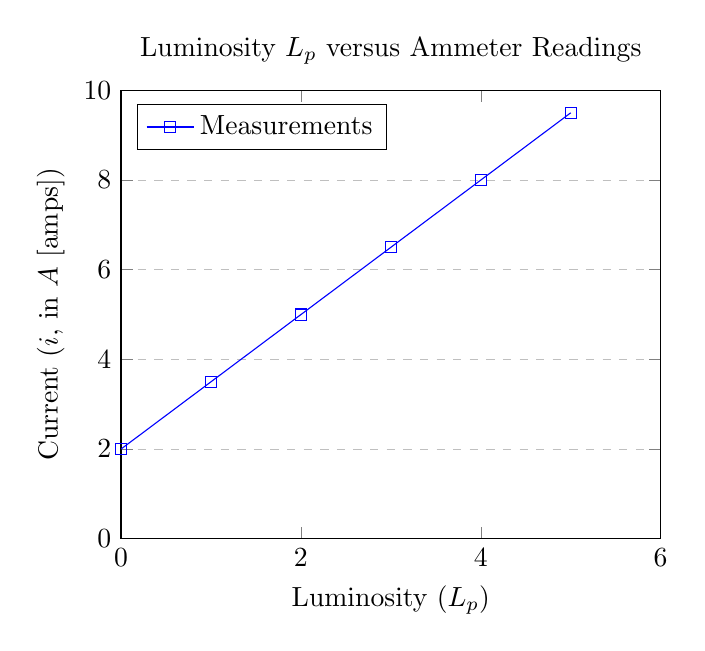
\begin{tikzpicture}
            \begin{axis}[
                title={Luminosity $L_p$ versus Ammeter Readings},
                xlabel={Luminosity ($L_p$)},
                ylabel={Current ($i$, in $A$ [amps])},
                xmin=0, xmax=6,
                ymin=0, ymax=10,
                xtick={0,2,4,6},
                ytick={0,2,4,6,8,10},
                legend pos=north west,
                ymajorgrids=true,
                grid style=dashed,
            ]
    
            \addplot[
                color=blue,
                mark=square,
                ]
                coordinates {
                (0,2)(1,3.5)(2,5)(3,6.5)(4,8)(5,9.5)
                };
                \legend{Measurements}
    
            \end{axis}
        \end{tikzpicture}
    \end{figure}
    \begin{enumerate}
        \item In the grid below, plot out the $i$ versus $V_p$ graph. Make sure to label at least 2 points on the graph.

        \note{
            Be sure to enforce the idea that in this class, for a fixed constant resistor, $I$ versus $V$ will always constant as well (the plot should always look like a slanted line with positive slope that passes through the origin). This is the essence of Ohm's Law and it won't be affected by any external settings (no matter how complicated they are).
        }

        \begin{figure}[H]
            \centering
            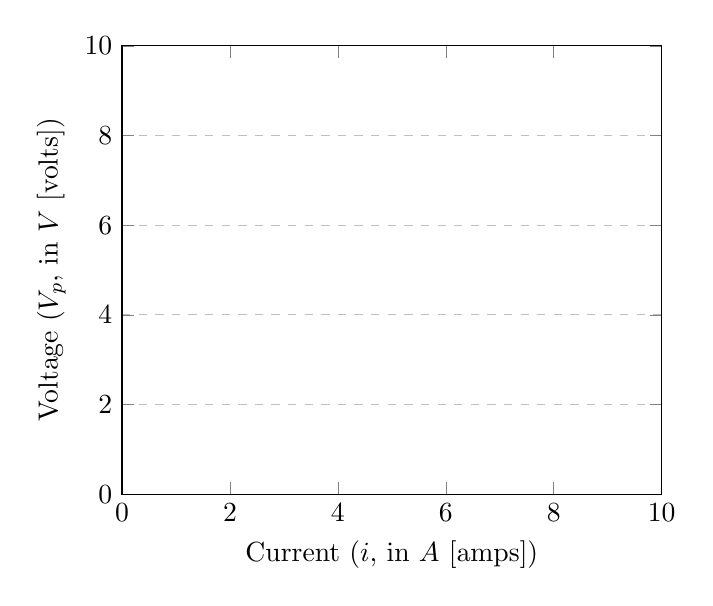
\begin{tikzpicture}
                \begin{axis}[
                    xlabel={Current ($i$, in $A$ [amps])},
                    ylabel={Voltage ($V_p$, in $V$ [volts])},
                    xmin=0, xmax=10,
                    ymin=0, ymax=10,
                    xtick={0,2,4,6,8,10},
                    ytick={0,2,4,6,8,10},
                    legend pos=north west,
                    ymajorgrids=true,
                    grid style=dashed,
                ]
                \end{axis}
            \end{tikzpicture}
        \end{figure}

        \sol{
        $V_p = i \cdot \frac{R_1R_2}{R_1 + R_2} = 1.2i$.

        \begin{figure}[H]
            \centering
            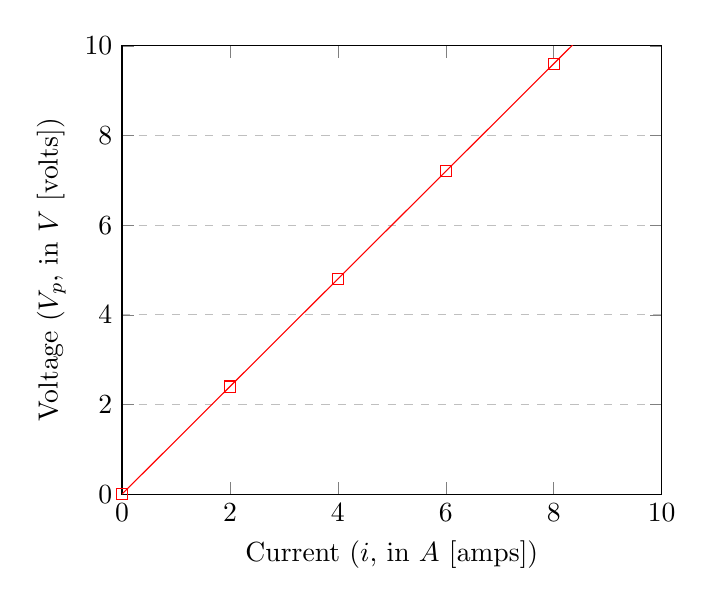
\begin{tikzpicture}
                \begin{axis}[
                    xlabel={Current ($i$, in $A$ [amps])},
                    ylabel={Voltage ($V_p$, in $V$ [volts])},
                    xmin=0, xmax=10,
                    ymin=0, ymax=10,
                    xtick={0,2,4,6,8,10},
                    ytick={0,2,4,6,8,10},
                    legend pos=north west,
                    ymajorgrids=true,
                    grid style=dashed,
                ]

                \addplot[
                color=red,
                mark=square,
                ]
                coordinates {
                (0,0)(2,2.4)(4,4.8)(6,7.2)(8,9.6)(10,12)
                };
                \end{axis}
            \end{tikzpicture}
        \end{figure}
        }
        \item Recover the expression for $V_p = f(L_p)$ based on the luminosity-v.s.-current plot.

        \sol{
            Observing the plot, we can derive $i$ as a function of $L_p$:
            $$i = 1.5L_p + 2$$
            Since we also know from analyzing the circuit in part 2 that:
            $$i = \frac{V_p}{R_1} + \frac{V_p}{R_2} = \frac{V_p}{1.2}$$
            Equating the two expressions, we have:
            $$\frac{V_p}{1.2} = 1.5L_p + 2$$
            And hence,
            $$V_p = f(L_p) = 1.2(1.5L_p + 2) = 1.8p + 2.4.$$
        }
    \end{enumerate}
\end{enumerate}

\end{document}